\newpage
\subsection{Almacenamiento}

Finalmente, los ángulos calculados por la red se almacenaron en un archivo. El formato para almacenar los archivos es el que muestra la Figura \ref{fig:formatoarchivo}.

\begin{figure}[htb]
	\centering
	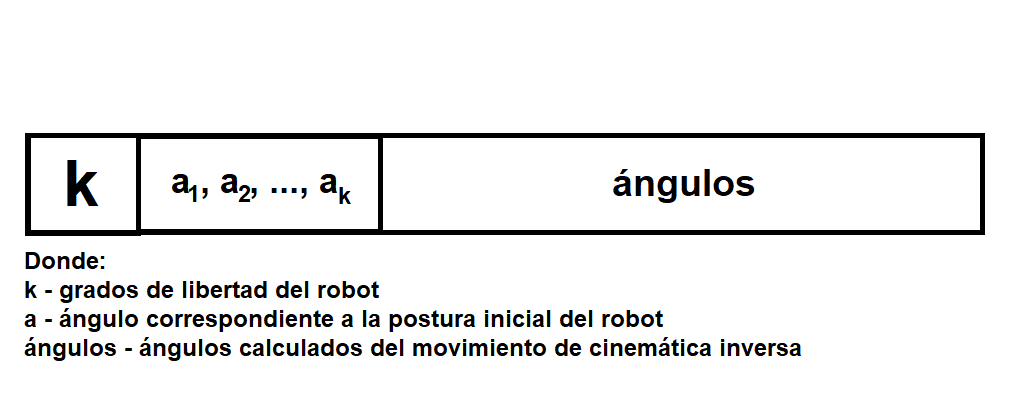
\includegraphics[scale=0.6]{formatoarchivo.png}
	\caption{Formato del archivo que guarda los datos de movimiento}
	\label{fig:formatoarchivo}
\end{figure}

El contenido del archivo se describe como sigue:

\begin{enumerate}
	\item El primer byte guarda la cantidad $k$ de ángulos de cinemática inversa calculados para el robot con $k$ grados de libertad
	\item Los siguientes $k$ bytes almacenan los ángulos de inclinación de la postura inicial del robot. Esta no necesariamente debe de corresponder con la postura inicial del brazo del operador, ya que lo que se controla en el brazo robótico, es el desplazamiento desde la posición inicial.
	\item El resto del contenido del archivo son los ángulos calculados para el problema de la cinemática inversa.
\end{enumerate}

De acuerdo con el mapa de registros \cite{registermap}, el tipo de dato del valor del ángulo de inclinación medido es de 2 bytes con signo. Esto quiere decir que el archivo aumenta en 18 bytes de información por cada instante en el que se mida la inclinación del dispositivo.